\chapter{バリデーション}
\section{実験概要}
\subsection{Video Cued-Recall メソッド}
インタラクティブ作品の評価方法にはさまざまな評価が存在するが、本作品を評価する上では、体験時、体験者がどのようなことに注意を向け、どのような行動を取ったかについて精緻に振り返る必要がある。そのため本研究では、体験者に体験時のようすをできるだけ詳細に表現してもらうため、Video Cued-Recallというメソッドを用いてデータの収集を行なった。 Video Cued-Recallとは、体験時のようすが記録された映像を視聴しながら、体験者本人が映像を手がかりに作品での体験を回顧し、言語化する方法である\cite{Costello2005}。インタビューを通して回顧するよりも詳細に体験を振り返ることができ、また体験しているそのときに体験のようすについて語ってもらう方法よりも、自然な体験について記述できることがその利点として挙げられる。

\subsection{参加者について}
インタビューは、FabCafe Nagoyaでの展示に際して、4名の体験者を対象に実施した。ただし、うち1名は「Relation」の体験時、トラッキングの精度が著しく低下していたため、1つ目に体験した「Familiar / Strange」の体験についてのみ調査の対象とした。

\subsection{データ収集}
参加者にはまず、調査の大まかな流れについて説明し、撮影についての許諾を得た。コンセプトの説明が自然な体験に影響することを避けるため、作品の体験の前にはコンセプトや具体的な作品の内容については説明せず、トラッキングされた手が次々に形を変えていくこと、手の形が表示された状態から始まり、再びもとの手の形に戻るループ構造のある作品であること、というインタビューに必要な最低限の構造のみ伝えた。

体験のようすは、手もとのハンドトラッキングを行うカメラ映像、現在時刻、体験者が実際に見ているスクリーンの映像が図\ref{fig:record_monitor}のようにレイアウトされて記録される。

\begin{figure}[H]
  \centering
  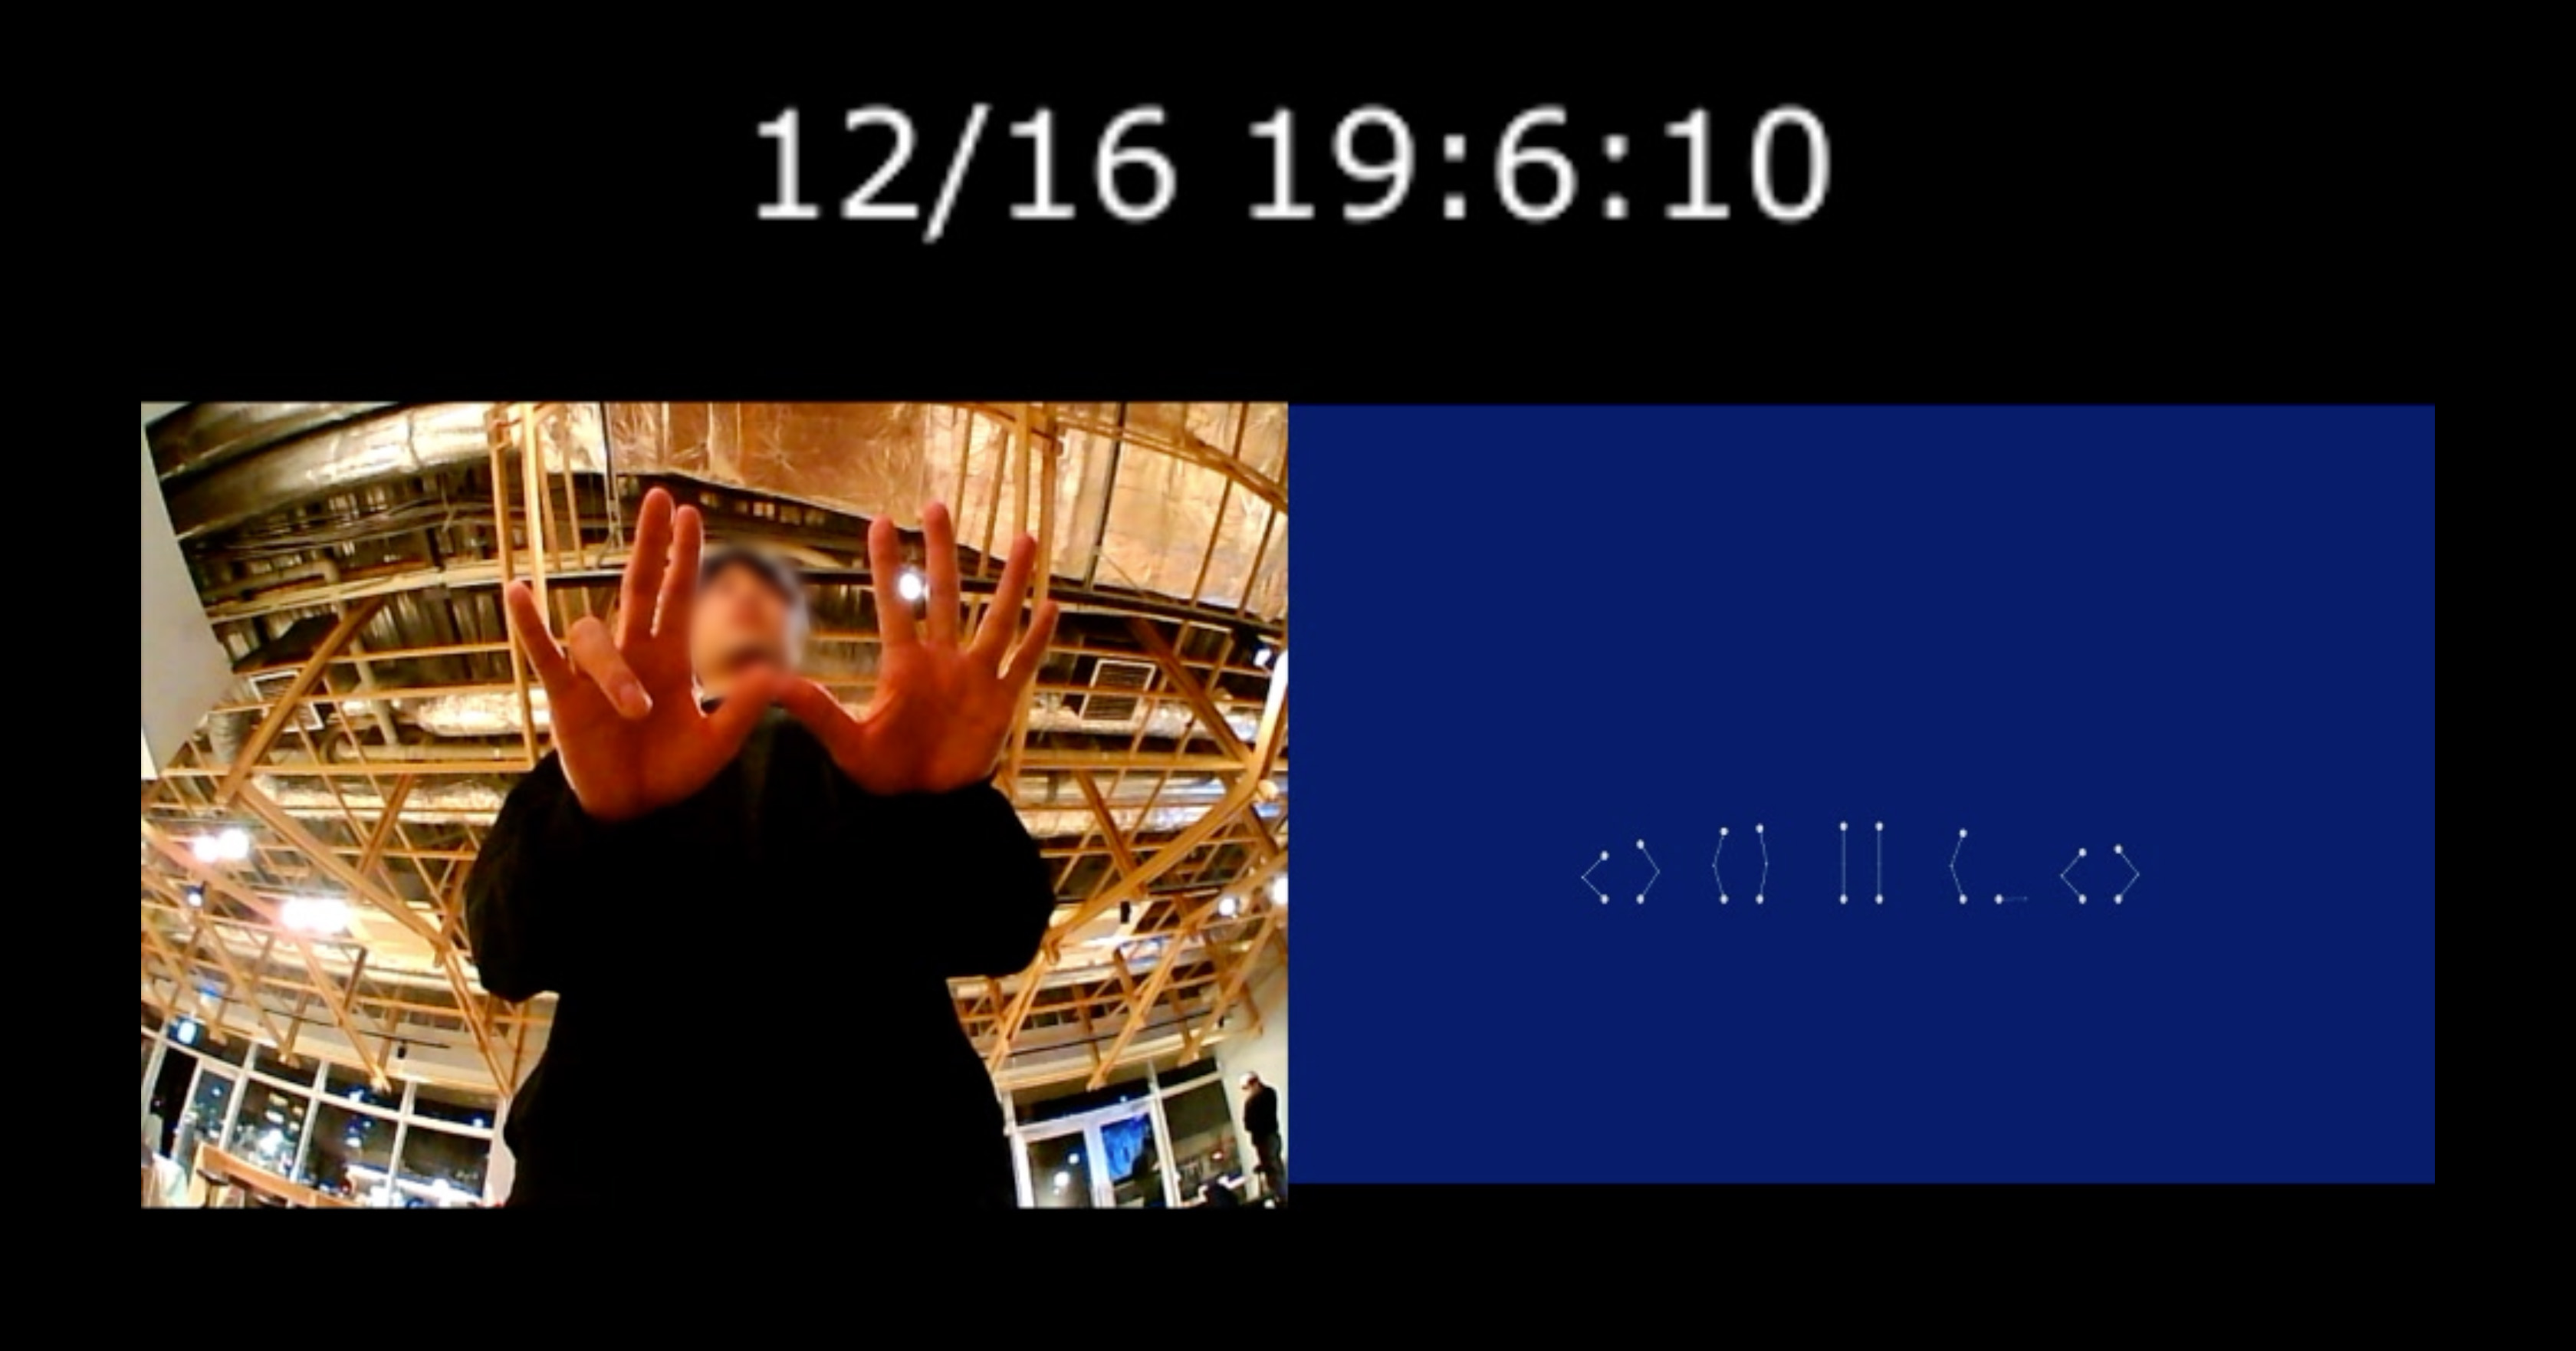
\includegraphics[width=15cm]{img/record_monitor.jpg}
  \caption{体験のようすの記録映像}
  \label{fig:record_monitor}
\end{figure}

作品体験が終了した後、体験者自身が上記の記録映像を視聴しながら、作品体験時のようすを詳細に言語化する振り返り作業を依頼する。この時点では、そのとき考えていたことや、試行した事柄とその理由など、作品体験を終えた今思う感想ではなく、その当時経験していたことについて言語化してもらうよう促した。体験者は、自由に映像を停止したり、巻き戻すことができる。
作業の際は研究実施者も同席しているが、調査を実施する上でのトラブルが生じない限り、原則体験者個人で振り返る。\\
その後、前の振り返りの作業や体験のようすを踏まえて、研究実施者が半構造化インタビューを実施することで、より精緻に作品体験のようすを振り返るとともに、体験を終えた上での感想などについて伺った。
いずれもループ構造の作品であるため、1周するまでの期間をその調査対象とした。ただし、作品「Relation」については、一周するための達成条件がシビアであることから、体験の終了は3分以上体験することを目安に、いつでも体験を終了してよいこととした。

\subsection{コーディング}
Video Cued-Recallを通して言語化された情報を、図\ref{fig:spreadsheet}のようにスプレッドシート上に時系列で記録した。シート上には、1秒ごとのタイムスタンプ(日本標準時)、その時刻でのトラッキングの状況(右手、左手、全体)、その時刻での出力内容を示すシーン情報、発言内容、並びに発言内容からその時点での体験者と作品との関係性を、Felsが定義した4つのカテゴリのうちのいずれかに割り振った結果が記録されている。
\begin{figure}[H]
  \centering
  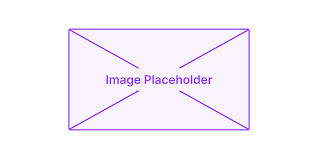
\includegraphics[width=15cm]{img/placeholder.png}
  \caption{発話情報が記録されたスプレッドシート}
  \label{fig:spreadsheet}
\end{figure}

\subsection{結果}
\subsubsection{Familiar / Strange}
全体的に、挙動を確認するための動きをする、すなわちResponseの動作をする参加者が多かった。
参加者4は、手の形が指ごとに分かれていくシーンで「ここら辺からちょっと違和感というか、親和性を確かめてたのに、その親和性から離れてく感じがしてた。今の自分の手と、こっち側の手の連動が、してるんだけど離れている。自分の手じゃなくなる。けど、なんか動いてる。こっちに合わせて動いてる、けどもうそれは手じゃないし、みたいな。」と語っていた。また、参加者5は、「最初はそうですね。このディスプレイに映ってるいろんな手の形を、トラッキングしたやつがどの手とリンクしているのかっていうのを確認というか、どれがどの場所なんだろうって、最初は手の形になっているのでわかるんだけど、まぁそれがずれていってどれがどれかなっていうのを結構確認してたかな。どれだっけ?みたいな感じで。」と語る。\\
さらに、体験の中でプリミティブな図像であるためか、何かしらの「見立て」をしていることが多いとわかった。参加者1は、指が縦方向の動きのみに拘束されてパタパタと上下する形になったときに、ピアノの演奏のような身体感覚を想起していた。また参加者4は、「頭の中で既視感を作って」体験していたと振り返る。\\
何かしら参照できる他の身体動作や、見立てが可能であることが、体験の中で目的意識や注意を自分で作って体験することにつながるのではないかと語っている。
一方で参加者3は、手でフレームを作るような動きをしており、それに対して画面の中の手は思うように形ができず、「途中から飽きていた」と語っていた。
指一本一本の単位で手指の構造が切り替わっていく構成ではあったが、そうした画面の変化について「認知が追いつかなかった」と振り返り、手指を使って形を作っていたというイメージに対して、画面の中の振る舞いがそれとは全く異なることについて注意が向かなかったのではないかと考える。
さらに、「思い通りに動く」とは「連動性が担保されていること」ではないか、という仮説が新たに生じた。
\subsubsection{Relation}
興味深いのは、体験におけるもどかしさについてはトラッキングの精度とはあまり関係していないという点である。\\
参加者1は、。また参加者3は、
これは、初めて体験する人にとって、トラッキングが途切れていることがもどかしさとして経験されるほど、Intimacyは高まっていないということが示唆される。
参加者1は、